\documentclass{article}
\usepackage{hw_style}
\usepackage{enumerate}
\usepackage{graphicx}
\usepackage{verbatim}

% Homework Specific Information
\newcommand{\hmwkTitle}{Homework \#2}
\newcommand{\hmwkDueDate}{September 9th, 3:00PM}
\newcommand{\hmwkAuthorName}{Kurt Rudolph}%Name:
\newcommand{\hmwkNetID}{rudolph9}%your netid
\newcommand{\hmwkNotes}{}%I worked with...

\newcommand{\hmwkSubTitle}{}
\newcommand{\hmwkClass}{STAT 400}
\newcommand{\hmwkClassTime}{}
\newcommand{\hmwkClassInstructor}{Yinxiao Huang}

\begin{document}
\begin{spacing}{1.1}
\maketitle
%=============================Problem1==========================%	
\newpage
\begin{homeworkProblem}
		Bob is applying for a job with five companies.  At the first company, he is in the final group of four applicants, one of which will be chosen for the position.  At two of the five companies, Bob is one of ten candidates; and at the last two companies, he is in an early stage of application in a pool of 25 candidates.  Assuming that all companies make their decisions independently of each other, and that Bob is as likely to be chosen as any other applicant, what is the probability of getting at least one job offer	
		
	\begin{homeworkSection}{Solution}
		Independent probability Bob gets a job at each compony accordingly:
		\[\frac{1}{4},\frac{1}{{10}},\frac{1}{{10}},\frac{1}{{25}},\frac{1}{{25}}\]
		Probability Bob gets a job at none of these companies: 
		\[\frac{3}{4} \cdot \frac{9}{{10}} \cdot \frac{9}{{10}} \cdot \frac{{24}}{{25}} \cdot \frac{{24}}{{25}} \approx 0.56\]
		Probability Bob gets a job at one or more companies:
		\[1 - 0.56 = 0.44\]
		
		
	
	\end{homeworkSection}
\end{homeworkProblem}
%===========================Problem2===========================%
\begin{homeworkProblem}
	At \emph{Initech}, 50\% of all employees surf the Internet during work hours.  20\% of the employees surf the Internet and play \emph{Solitaire} during work hours.  It is also known that 60\% of the employees either surf the Internet or play \emph{Solitaire} (or both) during work hours. 

	\begin{enumerate}[(a)]
		\item What proportion of the employees play \emph{Solitaire} during work hours?
			\begin{homeworkSection}{Solution}
				\[P(surfOnly) = P(surf) - P(surfAndSolitaire) = 0.50 - 0.20 = 0.30\]
				\[P(solitaire) = P(solitaireSurfOrBoth) - P(surfOnly) = 0.60 - 0.30 = 0.30 \]
			\end{homeworkSection}
		\item If it is known that an employee surfs the Internet during work hours, what is the probability that he/she also plays \emph{Solitaire}? 
			\begin{homeworkSection}{Solution}
				\[ P(solitaire | surf) = \frac{P(surfAndSolitaire)}{P(surf)} = \frac{0.20}{0.50} = 0.40 \]
			\end{homeworkSection}
		\item Suppose an employee does not play \emph{Solitaire} during work hours.  What is the probability that he/she surfs the Internet?
			\begin{homeworkSection}{Solution}
				\[P(surf | solitaire') = \frac{P( surf \cap solitaire')}{P(solitaire')} = \frac{P(surfOnly)}{1-P(solitaire')} = \frac{0.30}{0.70} \approx 0.4286 \]
			\end{homeworkSection}
		\item Are events \{an employee surfs the Internet during work hours\} and \{an employee plays \emph{Solitaire} during work hours\} independent?{\bf Justify your answer.}
			\begin{homeworkSection}{Solution}
				No $P(surfAndSolitaire) \ne 0$, $P(surfAndSolitaire) = 0.20$ as stated in the problem.  
			\end{homeworkSection}
	\end{enumerate}
\end{homeworkProblem}
%===========================Problem3===========================%
\begin{homeworkProblem}	
	During two-and-a-half years of research, bio-psychologist Onur G�nt�rk�n discovered that when people kiss, they turn their heads to the right roughly twice as often as to the left. (G�nt�rk�n, O. Human behaviour: Adult persistence of head-turning asymmetry. Nature, 421, 711, (2003).)
	
	Suppose the probability that a person would turn his/her head to the right is 2/3 , and
the probability that a person would turn his/her head to the left is 1/3 . A couple is planning a kiss on Valentine�s day. Assume that their choice of which way to turn their heads is independent of each other.
	\begin{enumerate}[(a)]
		\item What is the probability that they would both turn their heads to the right (and kiss)?
			\begin{homeworkSection}{Solution}
				\[P(heTurnRight \cap sheTurnRight) = P(heTurnRight)*P(sheTurnRight) = \frac{2}{3} \cdot \frac{2}{3} = \frac{4}{9}\]
			\end{homeworkSection}
		\item What is the probability that they would bump noses (i.e., choose the opposite direction to turn their heads)?
			\begin{homeworkSection}{Solution}
				\[ P(bumpNoises) =\]
				\[ 1 - P\left(P\left(heTurnRight \cap sheTurnRight\right) \cup P\left(heTurnLeft \cap sheTurnLeft\right)\right) =\]
				\[ 1 - \left( \left(\frac{2}{3} \cdot \frac{2}{3}\right) +\left(\frac{1}{3} \cdot \frac{1}{3}\right) \right) = \frac{4}{9}\]
			\end{homeworkSection}
	\end{enumerate}
\end{homeworkProblem}	
%===========================Problem4===========================%
\begin{homeworkProblem}
	From a group of 16 male and 9 female armadillos, Noah must choose two to travel on his ark. Unable to distinguish between male and female armadillos, Noah must choose at random.
	\begin{enumerate}[(a)]
		\item Noah chooses the {\bf two} armadillos at random. Compute the probability that Noah gets two armadillos of the opposite sex (i.e., one male and one female armadillo).
			\begin{homeworkSection}{Solution}
				\[P(male \cap female) = P(maleThenFemale) + P(FemaleThenMale) = \frac{16}{25} \cdot \frac{9}{24} + \frac{9}{25} \cdot \frac{16}{24} = \frac{144}{600} + \frac{144}{600} = 0.48\]
			\end{homeworkSection}
		\item In order to improve his chances of selecting at least one male and one female armadillo, Noah decides to "cheat" and select {\bf three} armadillos to travel on his ark. Compute the probability that Noah gets at least one male and one female armadillo.	
			\begin{homeworkSection}{Solution}
				\[P(male \cap female) =\]
				\[P(maleThenFemale) + P(FemaleThenMale) +\]
				\[P(maleThenMaleThenFemale) + P(femaleThenFemaleThenMale)=\]
				\[\frac{16}{25} \cdot \frac{9}{24} + \frac{9}{25} \cdot \frac{16}{24} + \frac{16}{25} \cdot \frac{16}{24} \cdot \frac{9}{24} + \frac{9}{25} \cdot \frac{9}{24} \cdot \frac{16}{23} \]
			\end{homeworkSection}
	\end{enumerate}
\end{homeworkProblem}
%===========================Problem5===========================%
\begin{homeworkProblem}
Does a monkey have a better chance of rearranging

I I I L L N O S to spell I L L I N O I S

or

E E E E N N S S T to spell T E N N E S S E E ?
	\begin{homeworkSection}{Solution}
		A monkey has a better chance of rearranging I I I L L N O S to spell I L L I N O I S.  ILLINOIS is only eight character while TENNESSEE is nine.
	\end{homeworkSection}
\end{homeworkProblem}
%===========================Problem6===========================%
\begin{homeworkProblem}
An electronic device has four independent components. Two of those four are new, and have a reliability of 0.80 each, one is old, with 0.75 reliability, and one is very old, and its reliability is 0.50.
	\begin{enumerate}[(a)]
		\item Suppose that the device works if all four components are functional. What is the probability that the device will work when needed?
			\begin{homeworkSection}{Solution}
				\[P(work) = 0.80*0.80*0.75*0.50 = 0.24\]
			\end{homeworkSection}
		\item Suppose that the device works if at least one of the four components is functional. What is the probability that the device will work when needed?
			\begin{homeworkSection}{Solution}
				\[ P(work \ge 1) = 1 - P(Work' = 4) = 1 - (0.20 * 0.20 * 0.25 * 0.50) =  0.95\]
			\end{homeworkSection}
		\item Suppose that the four components are connected as shown on the diagram below. Find the reliability of the system.\\
			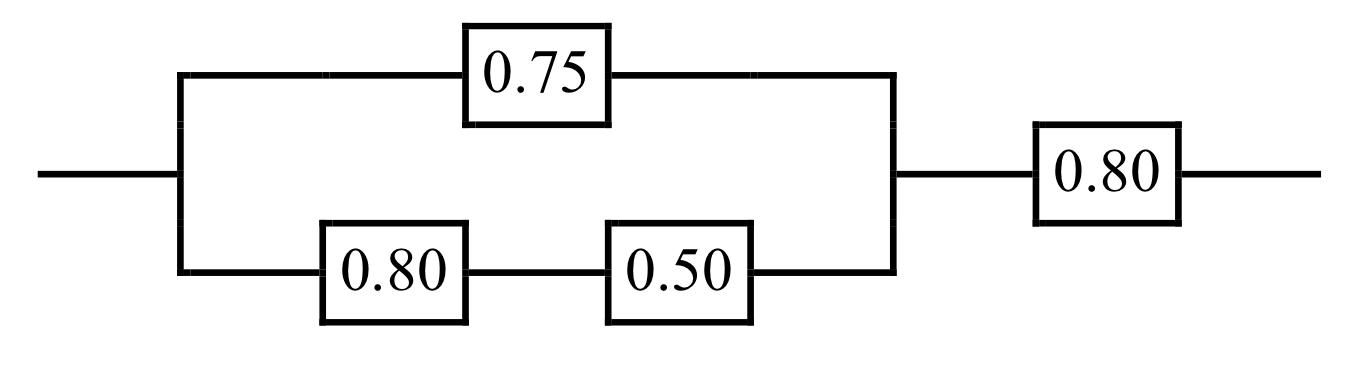
\includegraphics[width=\linewidth]{prob6.png}
			\begin{homeworkSection}{Solution}
				\[ P(work) = P(topBarWork \cup bottomBarWork) \cap P(endWork) =\]
				\[ (1 - P(topBarWork' \cap bottomBarWork')) \cap P(endWork) =\]
				\[ (1 - (0.25* 0.60))*.80 = 0.68\] 
			\end{homeworkSection}
	\end{enumerate}
\end{homeworkProblem}
%===========================Problem7===========================%
\begin{homeworkProblem}
	Three prisoners, $A$, $B$ and $C$, are in separate cells and sentenced to death. The governor has selected one of them at random to be pardoned. The warden knows which one is
pardoned, but is not allowed to tell. Prisoner A begs the warden to let him know the identity of one of the others who is going to be executed. "If $B$ is to be pardoned, give me $C$'s name. If $C$ is to be pardoned, give me $B$'s name. And if I'm to be pardoned, flip a coin to decide whether to name $B$ or $C$."
	
	The warden tells $A$ that $B$ is to be executed. Prisoner A is pleased because he believes that his probability of surviving has gone up from 1/3 to 1/2, as it is now between him and $C$. Prisoner $A$ secretly tells $C$ the news, who is also pleased, because he reasons that A still has a chance of 1/3 to be the pardoned one, but his chance has gone up to 2/3. What is the correct answer?
	\begin{homeworkSection}{Solution}
		Both $B$ and $C$ have equal probability of begin chose:
		\[ P(B_{picked}) = P(C_{pardoned}) \cup (P(A_{pardoned}) \cap P(B_{coinToss})) = \frac{1}{3} + \left( \frac{1}{3} \cdot \frac{1}{2} \right) = \frac{1}{2} \]
		\[ P(C_{picked}) = P(B_{pardoned}) \cup (P(A_{pardoned}) \cap P(C_{coinToss})) = \frac{1}{3}+ \left( \frac{1}{3} \cdot \frac{1}{2} \right) = \frac{1}{2} \]
		\[ \Rightarrow \]
		\[ P(A_{pardoned} | B_{picked}) = 
			\frac{P \left( P\left(A_{pardoned}\right) \cap P\left(B_{picked}\right)\right)}{P(B_{picked}) } = \]
			\[ \frac{ \frac{1}{3} \cdot \frac{1}{2}}{ \frac{1}{2}} = \frac{1}{3} \]
		\\ \[ P(B_{pardoned} | B_{picked}) 
			\frac{P \left( P\left(B_{pardoned}\right) \cap P\left(B_{picked}\right)\right)}{P(B_{picked}) } = \]
			\[ \frac{ \frac{1}{3} \cdot \frac{1}{2}}{ \frac{1}{2}} = \frac{1}{3} \]
		\\ \[ P(C_{pardoned} | B_{picked}) 
			\frac{P \left( P\left(C_{pardoned}\right) \cap P\left(B_{picked}\right)\right)}{P(B_{picked}) } = \]
			\[ \frac{ \frac{1}{3} \cdot \frac{1}{2}}{ \frac{1}{2}} = \frac{1}{3} \]
	\end{homeworkSection}
\end{homeworkProblem}

%===========================Problem8===========================%
\begin{homeworkProblem}
	{\bf 1.3-4} In designing an experiment, the researcher can often choose many different levels of the various factors in order to try to find the best combination at which to operate.  As an illustration, suppose the researcher is studying a certain chemical reaction and can choose four levels of temperature, five different pressures, and two different catalysts.  
	\begin{enumerate} [(a)]
		\item To consider all possible combinations, how many experiments would need to be conducted?
			\begin{homeworkSection}{Solution}
			
			\end{homeworkSection}{Solution}
		\item Often in preliminary experimentation, each factor is restricted to two levels.  With the three factors noted, how many experiments would need to be run to cover all possible combinations with each of the three factors at two levels?  (Note: this often called a 2 design).  
			\begin{homeworkSection}{Solution}
			
			\end{homeworkSection}{Solution}
	\end{enumerate}
\end{homeworkProblem}

%=============================Problem9==========================%	
\begin{homeworkProblem}
	{\bf 1.3-6} The "eating club" is hosting a make-your-own sundae at which the following are provided: 
	\\Ice Cream Flavors:
		\begin{itemize}
			\item Chocolate
			\item Cookies-n-cream
			\item strawberry
			\item Vanilla
		\end{itemize}
	Toppings:
		\begin{itemize}
			\item Carmel
			\item Hot fudge
			\item Marshmallow
			\item M\&M's
			\item Nuts
			\item Strawberries
		\end{itemize}
	\begin{enumerate}[(a)]
		\item How many sundaes are possible using one flavor of ice cream and three different toppings? 
			\begin{homeworkSection}{Solution}
				\[ \left| allFlavors \right| \cdot  \frac{ \left| allToppings \right| ! }{\left( \left| allToppings \right| - \left| toppings \right| \right)! }  = 4 \cdot \frac{6!}{3!} = 8 \]
			\end{homeworkSection}
		\item How many sundaes are possible using one flavor of ice cream and from zero to six toppings?
			\begin{homeworkSection}{Solution}
				
			\end{homeworkSection}
		\item How many different combinations of flavors of three scoops of ice cream are possible if it is permissible to make all three scoops the same flavor?
			\begin{homeworkSection}{Solution}
		
			\end{homeworkSection}
	\end{enumerate}	
\end{homeworkProblem}
%=============================Problem10==========================%	
\begin{homeworkProblem}
	{\bf 1.5-8}  Die $A$ has orange on one face and blue on five faces, Die $B$ has orange on two faces and blues on four faces, Die $C$ has $orange$ on three faces and $blue$ on three faces.  All are unbiased dice.  If the three dice are rolled, find the probability that exactly two of the three dice come up $orange$.  
	\begin{homeworkSection}{Solution}
		
	\end{homeworkSection}
\end{homeworkProblem}
%=============================Problem11==========================%	
\begin{homeworkProblem}
	{\bf 1.5-16} An urn contains five balls, one marked $WIN$ and four marked $LOOSE$.  You and another player take turns selecting a ball at random from the urn, one at a time.  The first person to select the $WIN$ ball is the winner.  If you draw first, find the probability that you will win if the sampling is done.  
	\begin{enumerate}[(a)]
		\item With replacement.
			\begin{homeworkSection}{Solution}
		
			\end{homeworkSection}
		\item Without replacement.
			\begin{homeworkSection}{Solution}
		
			\end{homeworkSection}
	\end{enumerate}
	
\end{homeworkProblem}
%=============================Problem12==========================%	
\begin{homeworkProblem}
	{\bf1.6-8} A store sells four brands of DVD players.  The least expensive brand, $B_1$, accounts for $40\%$ of the sales.  The other brands (in order of their price) have the following percentages of sales: $B_2$, $30\%$; $B_3$, $20\%$; and $B_4$, $10\%$.  The respective probability of needing repair during warranty are $0.10$ for $B_1$, $0.05$ for $B_2$, $0.03$ for $B_3$, and $0.02$ for $B_4$.  A randomly selected purchaser has a DVD player that needs repair under warranty.  What are the four conditional probabilities of being brand $B_i, i = 1,2,3,4$?
	\begin{homeworkSection}{Solution}
		
	\end{homeworkSection}
\end{homeworkProblem}
%=============================Problem13==========================%	
\begin{homeworkProblem}
	{\bf 1.6-10} Suppose we want to investigate the percentge of abused children in a certain population.  To do this, doctors examine some of these children take at random from that population.  However, doctors are not perfect: They sometimes classify an abused child $(A)$ as one not abused $(ND)$ or they classify a nonabused child $(N)$ as one that is abused $(AD)$.  Suppose theses error rates are $P(ND | A) = 0.08$ and $P(AD | N) = 0.05$, respectively; thus, $P(AD | A) = 0.92$ and $P(ND | N) = 0.95$ are the probabilities of the corrected decisions.  Let us pretend that only 2 percent of all children are abused; that is, $P(A) = 0.02$ and $P(N) = 0.98$.  
	\begin{enumerate}[(a)]
		\item  Select a child at random.  What is the probability that the doctor classifies this child as abused.  That is, compute 
			\[P(AD) = P(A) P(AD | A) + P(N) P(AD| N) \]
			\begin{homeworkSection}{Solution}
				
			\end{homeworkSection}
		\item Given that the child is classified by the doctor as abused, compute $P(N | AD)$ and $P(A | AD)$.  
			\begin{homeworkSection}{Solution}
		
			\end{homeworkSection}
		\item  Also, compute P(N | ND)  and P(A | ND).  
			\begin{homeworkSection}{Solution}
		
			\end{homeworkSection}
		\item Are the probabilities in (b) and (c) alarming?  This happens because the error rates of $0.08$ and $0.05$ are high relative to the fraction $0.02$ of abused children in the population.  
			\begin{homeworkSection}{Solution}
		
			\end{homeworkSection}
	\end{enumerate}
\end{homeworkProblem}
%=============================Problem14==========================%	
\begin{homeworkProblem}
	{\bf 2.1-10} Suppose there are 3 defective items in a lot (collection) of 50 items.  A sample of size 10 is taken at random and without replacement.  Let $X$ denote the number of defective items in the sample.  Find the probability that the sample contains. 
	\begin{enumerate}[(a)]
		\item Exactly one defective item.
			\begin{homeworkSection}{Solution}
		
			\end{homeworkSection}
		\item At most one defective item.  
			\begin{homeworkSection}{Solution}
		
			\end{homeworkSection}
	\end{enumerate}
	
\end{homeworkProblem}
%=============================Problem15==========================%	
\begin{homeworkProblem}
	{\bf 2.1-14} Often in buying a product at a supermarket, there is a concern about the item being underweight.  Suppose there are 20 "one-pound" packages of frozen ground turkey on display and 3 of them are underweight.  A consumer group buys 5 of the 20 packages at random.  What is the probability of at least 1 of the 5 being underweight?
	\begin{homeworkSection}{Solution}
		
	\end{homeworkSection}
\end{homeworkProblem}

\end{spacing}
\end{document}

\begin{comment}%%%%%%%%%%%%%%%%%%%%%%%%%%%%%%%%%%%%%%%%%%%
%=============================Problemi==========================
\newpage
\begin{homeworkProblem}
	
	\begin{homeworkSection}{Solution}
		
	\end{homeworkSection}
\end{homeworkProblem}
%=============================Problemi==========================%	
\begin{homeworkProblem}
	
	\begin{homeworkSection}{Solution}
		
	\end{homeworkSection}
\end{homeworkProblem}
%=============================Problemi==========================%	
\begin{homeworkProblem}
	
	\begin{enumerate}[(a)]
		\item 
			\begin{homeworkSection}{Solution}
		
			\end{homeworkSection}
	\end{enumerate}
	
\end{homeworkProblem}

\end{comment}%%%%%%%%%%%%%%%%%%%%%%%%%%%%%%%%%%%%%%%%%%%













